%------------------------------------------------------------------------------
% physor2016_template.tex - template to write a contribution for the PHYSOR 
% 2016 conference
% v2.0 20150508 Wilfred van Rooijen, University of Fukui
% v1.0 20130422 Wilfred van Rooijen, University of Fukui
%------------------------------------------------------------------------------
% Usage: this template file should be used ONLY with pdfLaTeX. Place this 
%        template file and the file physor2016.sty in the your working
%        directory. If you use bibtex, put physor2016.bst and physor2016.bib 
%        also in the working directory. If you have your own BiBTeX database
%        file, make a copy or link in your working directory and replace 
%        \bibliography{physor2014} with \bibliography{your_bib_file}.
%
% NOTE: when compiling your document, you may get warnings regarding
%       the versions of several of the style files used in the PHYSOR2016 tem-
%       plate. A warning is issued if the version on your computer is older than
%       the version requested in the style file. Under normal circumstances, 
%       there should be no problems but when in doubt, please check the log file
%       and update your LaTeX distribution if necessary. 
%------------------------------------------------------------------------------
\documentclass[12pt]{article}
%
% NOTE: use \documentclass[12pt,draft]{article} for your initial work. This 
%       will give you the "draft" mode:
%       - a black marker is printed for each "overfull hbox" (*)
%       - figures are not included (only the BoundingBox is indicated)
%       - hyperref is switched off
%
% (*) In LaTeX, the text is typeset on the paper per paragraph - this is quite
%     different from MS Word where the text is typeset line-by-line. TeX will 
%     try to find an "optimal" layout of the paragraph. TeX uses "penalties" for
%     situations which are not optimal. TeX keeps re-setting the paragraph until 
%     the total penalty is minimized. To make an optimal layout, TeX uses line
%     breaking (hyphenation) and "spacing". For example, TeX can increase or de-
%     crease the space between words to fill out a line; in fact, TeX even 
%     allows to change the spacing between letters in a word - this is called
%     "kerning".
%     To make an optimal page layout, the line spacing is variable, and also
%     the spacing between paragraphs. In TeX vocabulary, these spaces are known
%     as "rubber lengths".
%     But sometimes TeX gets confused. For example, if you use very long words
%     and TeX cannot determine the proper hyphenation, of if you have an 
%     "inline" math section (an expression between $...$). In that case, 
%     there is no proper hyphenation. If the word is not too long, TeX will keep
%     the word on the line, but there will be "too many words" on the line; this
%     is known as "overfull hbox", and the last word will protrude into the 
%     right margin.  
%     If the word is really long, TeX will move the word to the next line, but
%     then the previous line will have "not enough words"; this is known as
%     "underfull". 
%     Both overfull and underfull boxes are not very satisfactory. TeX prints
%     the warnings into the log file. If the "draft" mode is on, then there 
%     will be a visible reminder in the PDF file of overfull and underfull 
%     boxes.
%
%     To prevent underfull / overfull boxes, basically you need to give TeX more
%     "options" to properly fill the line: 

%     - add hyphenation locations in long words: hy\-phe\-na\-tion
%     - rewrite the sentence so that the long word or the equation is not at
%       the end of the line
%     Try to get rid of all the underfull and overfull boxes - but sometimes a
%     it just can't be avoided. 
%
\usepackage{physor2016}
%
% The basic style file loads a minimum of other style files. If you need special 
% styles, simply include them here. For example, you may be interested in the
% following packages:
%
% For anything that involves mathematics, equations, etc
%
\usepackage{amsmath}
%
% For real, bold face mathematical symbols
%
\usepackage{bm}
%
% To include figures in your paper. Note the following: manuscripts must be
% prepared in PDF. To do this, use pdflatex to produce PDF directly. pdflatex
% can include figures in the following formats: PDF, JPG, and PNG. For bitmap-
% ped images (photos etc), JPG is the preferred format, because JPG images can 
% be compressed very well in PDF, giving very small PDF files. For graphs and 
% schematics, vector images should be used; these can be either PostScript or
% PDF. If you have your figures as (e)ps, then see the notes at the end of this
% file for how to convert (e)ps to pdf. Note: bitmapped images should have
% a resolution of at least 300x300 dpi. For example, if your image has a size 
% of 1200x900 pixels, it should occupy not more than 4"x3" (approx 10x7.5 cm)
% in the manuscript. If you have many, large sized bitmap images which are 
% included with small size in the manuscript, then consider to re-size the 
% images before inclusion to maintain a reasonable size of the final PDF file.
%
% Making PDF images with Excel: use the Microsoft "save as PDF" plugin in 
% MS Office, and use the options of this plugin to export only one figure from
% you Excel file.
%
% To make very pretty diagrams etc with LaTeX, check out PGF/TikZ
%
\usepackage{graphicx}
\usepackage{tikz}
\usepgflibrary{shapes.geometric}
%
% If you use a table, check out this package. It creates tables with a little
% bit more space around the table entries. The result is a table that is easier
% to read, especially if you have mathematical super/subscripts in your work.
% Also check the manual of the package booktabs because it has some good tips 
% on how to make beautiful and informative tables.
%
\usepackage{booktabs}
%
% The following package takes care of setting SI units. Simply type 
% \degreeCelsius instead of $^\circ$ C. Also takes care of exponents and powers 
% of ten, as well as lining out numbers on the decimal point if required
\usepackage{siunitx}
%------------------------------------------------------------------------------

%------------------------------------------------------------------------------
% Define title. Use all CAPITALS.
%------------------------------------------------------------------------------
\title{THIS IS THE TEMPLATE TO WRITE A MANUSCRIPT FOR PHYSOR~2016 WITH \LaTeX, THE TITLE SHOULD NOT EXCEED THREE LINES.}
%
% ...and authors
%
\author{ 
  \textbf{First A. Author and Second B. Author\footnote{You can use foot notes if needed, for instance to include the address of your homepage: \href{http://www.nce.upalookaville.edu/}{www.nce.upalookaville.edu}}} \\
  Department of Nuclear \& Chemical Engineering \\
  University of Palookaville, Palookaville, New Jersey, USA\\
  \href{mailto:f.a.author@upalookaville.edu}{f.a.author@upalookaville.edu}\\
  \href{mailto:s.b.author@upalookaville.edu}{s.b.author@upalookaville.edu}\\
  \\                       % Put an extra empty line for different affiliations 
  \textbf{Third Author\footnote{\href{http://www.harahira.co.jp/ned/}{www.harahira.co.jp/ned/}}} \\
  Nuclear Engineering Division \\
  Harahira Heavy Industry, Mihama, Fukui, Japan\\
  \href{mailto:author.third@harahira.co.jp}{author.third@harahira.co.jp}
}

%------------------------------------------------------------------------------
% The \shortauthor is printed on top of the even pages, and the \shorttitle
% is printed on top of the odd pages.
% Suggested format:
% - One author             : A. Author
% - Two authors            : A. Author \& B. Author
% - Three authors          : A. Author, B. Author \& C. Author
% - More than three authors: A. Author~et~al.
% If the title of your manuscript is very long, then make a short title such
% that it fits on one line in the header of the odd pages.
%------------------------------------------------------------------------------
\renewcommand{\shortauthor}      % Author's names here
           {Authors' names, use~et~al.~if more than 3}  
\renewcommand{\shorttitle}       % Short title here
           {Paper Title (shortened version to fit in a single line)}  

%------------------------------------------------------------------------------
% Setup PDF info. This sets several values which are listed as the "properties"
% of the PDF file.
%------------------------------------------------------------------------------
\hypersetup{
  pdftitle=\shorttitle,
  pdfauthor=\shortauthor
}

%------------------------------------------------------------------------------
% Begin document
%
% \doublespacing -- This option will increase the line spacing, making it 
%                   easier to add written comments etc. Be sure to switch it 
%                   off when you make the final version!
%
% \linenumbers -- switches on line numbers, which are practical when reviewing 
%                 a manuscript. Switch off line numbers when you make your 
%                 final version. 
%------------------------------------------------------------------------------
\begin{document}

%\doublespacing

%\linenumbers

%------------------------------------------------------------------------------
% Make the titlepage and set the pagestyle to fancy throughout
%------------------------------------------------------------------------------
\maketitle

\begin{abstract}
  Provide an informative abstract of about 200 - 250 words. The abstract should give a short overview of all material to be discussed in the paper, including the background and / or justification of the research, the research method(s), the main result(s) and the conclusion(s). From the information in the abstract the reader should be able to determine whether or not the paper (and the presentation) will be worthwhile to study.
\end{abstract}

\keywords{Provide at 3 keywords minimum, 6 keywords maximum}

%------------------------------------------------------------------------------
%
%------------------------------------------------------------------------------
\section{INTRODUCTION}
\label{sect::intro}

Section headers should be all capitals (upper case), such as illustrated above. In this section, I would like to explain how to write your name(s) on the title page of the manuscript. 

\emph{Format for personal name(s)}: The format to enter a personal name is different from country to country. We do not enforce any strict rules. Write your name(s) in the format that feels most natural to you. If desired, you can emphasize your family name by writing it in ALL CAPITALS. We do not specify specific rules for hyphenation and/or interpunction in names: ``Jean-Marie Leblanc", ``J.-M. Leblanc", or ``Leblanc, JM" are all equally acceptable. If there are two authors with the same affiliation, then use ``Author1 and Author2"; if there are three or more authors with the same affiliation, use ``Author1, Author2, ..., AuthorN, and AuthorN+1".

\emph{Address format:} Since the format of street addresses is different from country to country, we do not enforce any specific format. In fact, a street address is not necessary. We only require the following: for each (co-)author, an affiliation must be entered, and for the corresponding author, at least an email address must be provided. If one of the authors is retired then please state the affiliation as ``retired", or ``formerly affiliated with XYZ". If an author is otherwise unaffiliated, then please write ``unaffiliated". A street address is \emph{not required}, but may be entered if desired. If you decide to enter a street address, then give sufficient details, including ZIP code etc, and don't forget the name of the country. Feel free to add other contact details, such as home pages, etc.

%------------------------------------------------------------------------------
%
%------------------------------------------------------------------------------
\section{SECOND OR SUBSEQUENT MAJOR HEADING}
\label{sect::second}

It is up to the writer to divide the manuscript into sections and sub-sections. For a conference contribution, in general 2 levels of sectioning should be adequate (i.e. sections and sub-sections), but we allow subsub-sections. If you want to make an appendix, check Appendix~\ref{app::a} for details about the format.

%------------------------------------------------------------------------------
%
%------------------------------------------------------------------------------
\subsection{Subsection Title: First Character of Each Non-trivial Word is Uppercase}
\label{subsect::major}

\LaTeX\ has several classes of characters. For instance, there are normal letters, mathematical symbols, and special characters. White space is one of the special characters. In \LaTeX\, a white space does not have a constant width. Rather, the spacing between words is adjusted so that lines and paragraphs are optimally typeset\footnote{In fact, the space between letters in a word is also adjusted to give an optimal paragraph filling. The process of spacing the letters within a word is known as \emph{kerning}.}. A special case is the combination of a period (full stop, ``.") followed by whitespace. This indicates to \LaTeX\ a break between sentences and then it is allowed to stretch space even further. Also, whitespace is interpreted in \LaTeX\ as a potential location for a line break. But sometimes, you want to have some white space, but no line break: for example, when you make a Reference like ``Figure~XYZ``, you want to make sure that a line break does not happen between the ``Figure" and the ``XYZ". In that case, use the special ``unbreakable space": the tilde-sign \~~, i.e. use \verb|Figure~\ref{fig::figure}| instead of \verb|Figure \ref{fig::figure}|. Use this also for citations, i.e. use \verb|See~\cite{book}| and not \verb|See \cite{book}|. The same applies for the construction ``et~al.", where the space between ``et" and ``al." should be non-stretchable and non-breakable, i.e. \verb|et~al.|. If ``et~al." is used in a running sentence, then use \verb|et~al.~| to make sure that the space after the period is interpreted as a non-stretchable space.

%------------------------------------------------------------------------------
%
%------------------------------------------------------------------------------
\subsubsection{Sub-subsection: use italic font, only first word is capitalized} 
\label{subsubsect::minor}

You can use a sub-subsection if you need to.

%------------------------------------------------------------------------------
%
%------------------------------------------------------------------------------
\section{ANOTHER SECTION: MAKING REFERENCES} 
\label{sect::references}

The \texttt{physor2016} style uses the \texttt{natbib} package to improve the typesetting of references. In general, the normal citation should be sufficient, i.e. \verb|\cite{book}|. However, natbib has various citation commands and allows to put options into the citation command. See the natbib manual for more information. If you want to cite more than one work, simply combine them into one \verb|\cite{}|: \verb|\cite{book_A,book_B,article_Z,manual_X}|. The natbib package will make sure that the final typesetting is ``reasonable". With natbib, you get this: (see~\cite{proc_paper,website,journal,book}); rather than this: (see~\cite{proc_paper},~\cite{website},~\cite{journal},~\cite{book}). References should be listed in the order that they are called out in the text (note: this is automatic if you use Bib\TeX).

%------------------------------------------------------------------------------
%
%------------------------------------------------------------------------------
\subsection{Hyperlinks} 
\label{subsect::hyper}

The \texttt{physor2016} style uses the \texttt{hyperref} package to pretty-print URLs. URLs are a special category for typesetting. For example, the tilde-sign (\~) usually indicates unstretchable space in LaTeX, but in URLs it should be typeset ``as is". URLs may contain periods (``.") but these periods do not indicate the end of a sentence. Furthermore, URLs do not contain whitespace, and therefore URLs cannot be treated with the normal line breaking algorithms in \LaTeX. Besides, even if a URL is split over a line, then a hyphen-sign should not be inserted. The hyperref package takes care of these issues, as well as several other benefits:

\begin{itemize}
\item All references in your document become hyperlinks automatically. When you use a \verb|\ref{}|, the PDF document will have a hyperlink in place which allows you to navigate through your document. This feature is very practical for instance to refer to equations.

\item All bibliographic material is internally linked; one click on the link will show you the book.

\item In the author entry on the first page, the optional \verb|mailto:|-prefix can be used, and a hyperlink will be created. If this link is clicked, the default email editor is started and an email to the author is automatically initialized. Think of it as a service to your readers.
\end{itemize}

See the hyperref documentation if you want to know more. Please note that if you use the ``final" option when you compile your manuscript, the hyperlinks will be color-coded in the PDF file.

%------------------------------------------------------------------------------
%
%------------------------------------------------------------------------------
\section{EQUATIONS}
\label{sect::equations}

The full power of \LaTeX\ is in typesetting mathematical material. Please use the \texttt{amsmath} package. Note the following: \LaTeX\ provides the \texttt{equation}-environment and the \texttt{equation*}-environment. The starred version produces no equation number. According to tradition, an equation is only given a number if there is a reference to the equation. Indeed, if the equation is not refered to, there is no need for an equation number. But for the present template, strict numbering rules are not enforced. A simple equation:

\begin{equation*}
  a^2 + b^2 = c^2
\end{equation*}

But \LaTeX\ also allows very long equations, such as Equation~\eqref{eq::orig_trans}. Note: please use \verb|\eqref{}| to refer to equations.

\begin{multline}
  \hat \Omega \cdot \nabla \psi ( \vec r, E, \hat \Omega )  + \Sigma_t ( \vec r, E ) \psi ( \vec r, E, \hat \Omega ) = \\ \int \limits_{0}^{\infty} \! \int \limits_{4 \pi} \! \Sigma_s ( \vec r, E^\prime \rightarrow E, \hat \Omega^\prime \rightarrow \hat \Omega ) \psi ( \vec r, E^\prime, \hat \Omega^\prime ) \, \mathrm{d}\hat \Omega^\prime \, \mathrm{d}E^\prime + \\ \frac{\chi ( \vec r, E )}{4\pi} \int \limits_0^\infty \! \int \limits_{4\pi} \nu \Sigma_f ( \vec r, E^\prime ) \psi ( \vec r, E^\prime, \hat \Omega^\prime ) \, \mathrm{d} \hat \Omega^\prime \, \mathrm{d}E^\prime + S_\text{ext} ( \vec r, E, \hat \Omega ) \label{eq::orig_trans}
\end{multline}

Please always introduce all symbols in your equations, avoid things like ``all symbols have their conventional meaning". Another point about style is the typesetting of the the $d$ (or better, the $\mathrm{d}$) in differential equations. In order to clearly distinguish the ``differential-d" from a ``symbol-d", it is common practice to typeset the ``differential-d" upright. In \LaTeX, this can be achieved by using \verb|\mathrm{d}|. Consider the following equations to see the difference clearly:

\begin{equation*}
  \frac{dC_i}{dt} = \frac{\beta_i}{\Lambda} n(t) - \lambda_i C_i(t)
\end{equation*}

versus

\begin{equation*}
  \frac{\mathrm{d}C_i}{\mathrm{d}t} = \frac{\beta_i}{\Lambda} n(t) - \lambda_i C_i(t)
\end{equation*}

I would also like to draw your attention to the following: sometimes, boldface symbols are used in mathematical equations. \LaTeX provides a ``native" command to obtain boldface mathematical symbols: \verb|\mathbf{}|. However, this command does not always give the desired result. For example: \verb|$k~\text{vs}~\mathbf{k}$| gives the following result: $k~\text{vs}~\mathbf{k}$. Indeed, the $k$ became bold, but it also changed from a slanted shape to an upright shape. And \verb|$\phi~\text{vs}~\mathbf{\phi}$| will not give any result: $\phi~\text{vs}~\mathbf{\phi}$ - the symbol does not change at all. For these cases, use the bm package (bm stands for bold math). This package provides properly proportioned, bold face symbols for all mathematical symbols. You can see the difference clearly: \verb|$k~\text{vs}~\bm{k}$| results in: $k~\text{vs}~\bm{k}$, where the $k$ is bold face and still properly slanted, and \verb|$\phi~\text{vs}~\bm{\phi}$| gives: $\phi~\text{vs}~\bm{\phi}$.

%------------------------------------------------------------------------------
%
%------------------------------------------------------------------------------
\section{FIGURES AND TABLES} 
\label{sect::floats}

\LaTeX\ has many packages to make it easy to include figures into your manuscript. With pdf\LaTeX\, you can include figures as PDF, JPG, or PNG. For bitmapped material, JPG is preferred, because it can be compressed very efficiently into the PDF file and very small PDF files will result. For bitmapped images, please use a resolution of at least 300x300 dpi. For graphs and schematic drawings, please use PDF. This will provide so-called vector-images, which have a very small file size, and which provide optimal resolution under all magnification. To make very nice schematics in pdf\LaTeX\, check out PGF/TikZ. All figures and tables need to be refered to in the running text. Figures or tables without references (``dangling" figures and tables) are not allowed!

One of the issues with \LaTeX\ is that the size of the figure in the final document is not known, and you need several iterations to find the correct size. In general, you can avoid trouble by using the \texttt{[width=]}-option of the \verb|\includegraphics{}| command, in combination with the parameter \verb|\textwidth|. For example, to set two figures side-by-side and remain within the text width, use: 

\begin{verbatim}
  \includegraphics[width=0.45\textwidth]{foo1.pdf}
  \includegraphics[width=0.45\textwidth]{foo2.pdf}
\end{verbatim}

The result would be something like Figure~\ref{fig::sym6}. Obviously, this only works if both figures are roughly equal in size to begin with. See the manual of the graphicx package for more info. If you need to set several figures together, consider the subfigure package which allows to set complex combinations of small figures into one larger figure. 

\begin{figure}[ht!]
  \begin{center}
    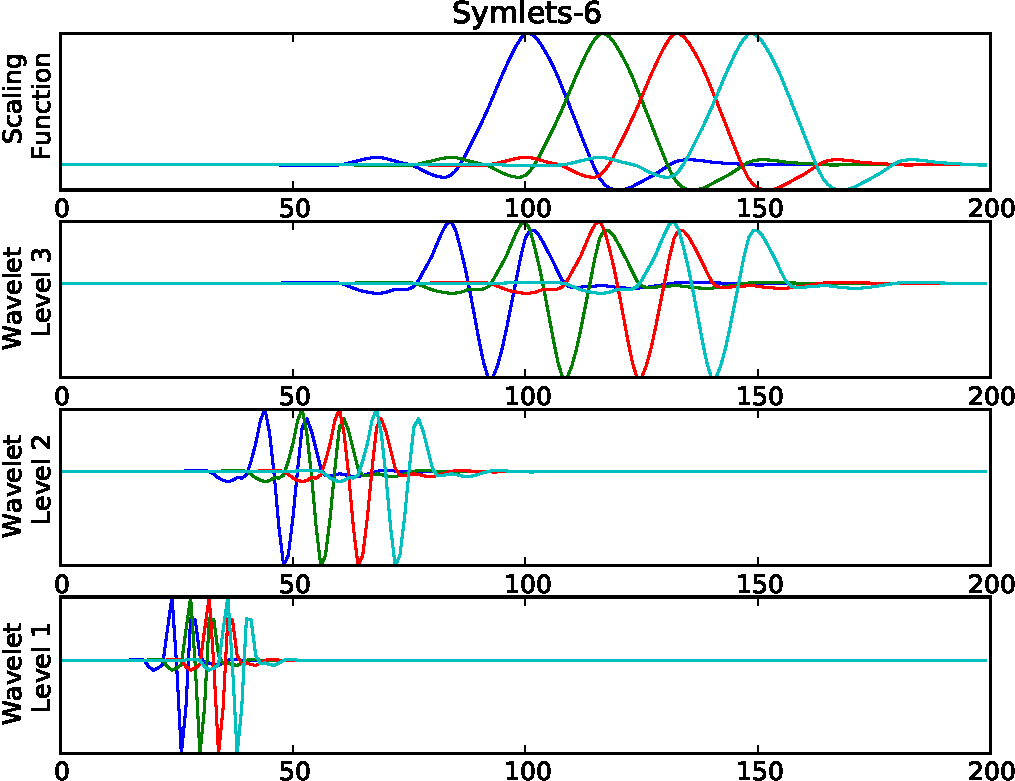
\includegraphics[width=0.45\textwidth]{sym6-crop.pdf}
    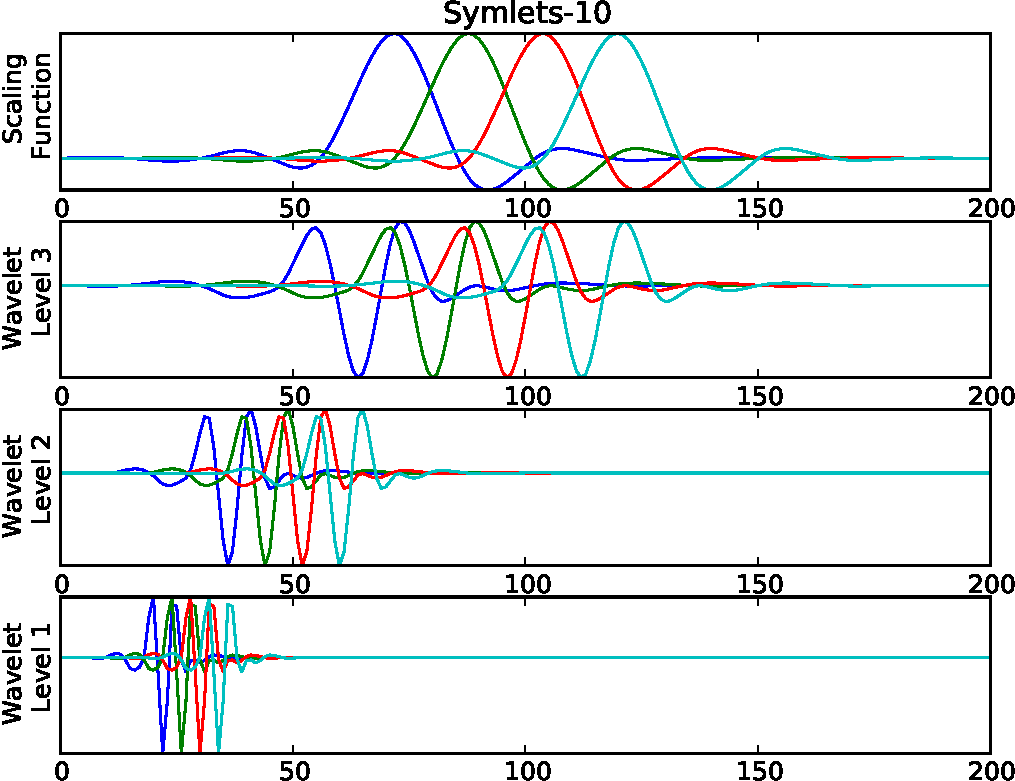
\includegraphics[width=0.45\textwidth]{sym10-crop.pdf}
    \caption[]{\label{fig::sym6}Figure captions go underneath the figure, over the full width of the page.}% Only the ``Figure" label and figure number are bold.}
  \end{center}
\end{figure}

Also note that figures and tables are, in \TeX-terminology, ``floating objects" (aka ``floats"). Floating objects are information to be put on the page, but the location of the material can be varied (within a certain range). In other words, when you put the \verb|\begin{figure}...\end{figure}| in your document, the figure will actually show up in a different location - and depending on your settings and the size of the figure, the float may end up on the very last page of the manuscript! This is due to the nature in which \TeX typesets the page. Floats are set with certain rules to give an ``aesthetically pleasing" result. \LaTeX provides an option to give the user a bit more control over the placement of floats: the so-called \verb|[htbp]|-specifier, which means ``place the float (h)ere, (t)op of page, (b)ottom of page, or separate (p)age". Thus, if you prefer you floats at the top of the page, then you can say \verb|\begin{figure}[t]...\end{figure}|. However, the process of optimization in \TeX still implies that the \verb|[htbp]|-specifier can be overridden. To give the user even more control, you can add an exclamation point: \verb|\begin{figure}[ht!]...\end{figure}|: put the figure here, or otherwise on the top of the page, and that's all the freedom there is. In this case, the placement may still be overridden by \TeX and an error will be written in the log file.

If a float is simply to large to fit onto a page, a message ``float too large for page" will be written in the log file. If this happens, please resize the float (perhaps with the \verb|width=...|-specifier) so that it fits on a page. If a float is extremely large, it will not fit an the present page, and \TeX will push it to the next page; on the next page, it will also not fit, and \TeX will push it to the next page; etc, etc.. In other words, if you have an extremely large float, it will end up on the very last page of the document!

For tables, we do not enforce any special style. Writers are encouraged to take a look at the booktabs package. The manual of this package has some interesting pointers to create beautiful and informative tables. An example of a table is given, see Table~\ref{tab::unc}.

\begin{table}[ht]
  \begin{center}
    \caption{\label{tab::unc}Table captions appear above the table, over the full width of the page. Only the ``Table" label and table number are bold.}
    \begin{tabular}{llll}
    \toprule
    Parameter & \multicolumn{2}{c}{Current uncertainty (LMFBR) [\%]} & Target uncertainty [\%]\\
              & Input data                & Modeling &                    \\
    \midrule
    $k_\text{eff}$          & 1.5 & 0.5 & 0.3 \\
    Power peak              & 1   & 3   & 2   \\
    Power distribution      & 1   & 6   & 3   \\
    Control rod worth       & 5   & 6   & 5   \\
    (element)               &     &     &     \\
    Control rod worth       & 5   & 4   & 2   \\
    (total)                 &     &     &     \\
    Reactivity coefficients & 7   & 15  & 7   \\
    (total)                 &     &     &     \\
    Reactivity coefficients & 20  & 20  & 10  \\
    (component)             &     &     &     \\
    Decay heat              & 10  & 3   & 5   \\
    \bottomrule
    \end{tabular}
  \end{center}
\end{table}

%------------------------------------------------------------------------------
%
%------------------------------------------------------------------------------
\section{A SECTION WITH A BITMAP IMAGE} 
\label{sect::bitmap}

It is an age-old debate: which is faster, a Formula-1 car or a Formula-1 motorcycle? Technically, there is no Formula-1 in motorcycle road racing. The fastest category is known as \emph{MotoGP}. Surely, the motorcycle is much lighter than the car, and since it has a powerful engine, it has a very good power-to-weight ratio. Therefore, one expects that the motorcycle is faster. However, both the car and the motorcycle are subject to physics. The maximum acceleration and deceleration are governed by the maximum torque that can be transmitted through the tyres to the road surface. If this torque is exceeded, the following occurs:

\begin{itemize}
\item In the case of the F1 car, the wheels will either spin (acceleration), or the wheels will lock up (deceleration).

\item In the case of acceleration of the motorcycle, the torque will cause the front wheel to come off the ground: a \emph{wheelie}. The required torque to cause a wheelie is related to the distance between the rear wheel and the center of gravity of the motorcycle: the longer the distance, the higher the maximum torque. When the front wheel comes off the ground, the distance between the center of gravity and the rotation axis of the rear wheel becomes shorter (the center of gravity rotates around the real wheel). Thus, if the rider does not reduce the throttle, the wheelie will escalate and the motorcycle will make a backflip.

\item Upon hard braking on the motorcycle, the opposite of a wheelie occurs. This is known as a \emph{stoppie}. In this case, the center of gravity rotates around the front wheel, and if the driver does not reduce the brake pressure, the motorcycle will flip over the front wheel.

\item Of course, in the case of the motorcycle there is also the problem of the adhesion of the tyre rubber to the road surface. For example, under wet conditions, a wheelie or a stoppie is unlikely because the rubber will lose grip before a wheelie (stoppie) can occur.
\end{itemize}

Both a wheelie and a stoppie are illustrated in Figure~\ref{fig::wheelie}. In practice, the F1 car can transfer more torque to the road surface, because the distance between the wheel axles and the center of gravity is bigger. Also, the wheels of the car provide a much bigger contact surface area and therefore more adhesion to the road surface. For these reasons, the F1 car can sustain much larger acceleration (deceleration) than the motorcycle, and as a result, the F1 car is (much) faster on the track. When expressed in numbers, the difference is striking. For example on the Suzuka Circuit in Japan, the fastest lap time for an F1 car 1:31.540, and for motorcycles 2:07.110.

\begin{figure}
  \begin{center}
    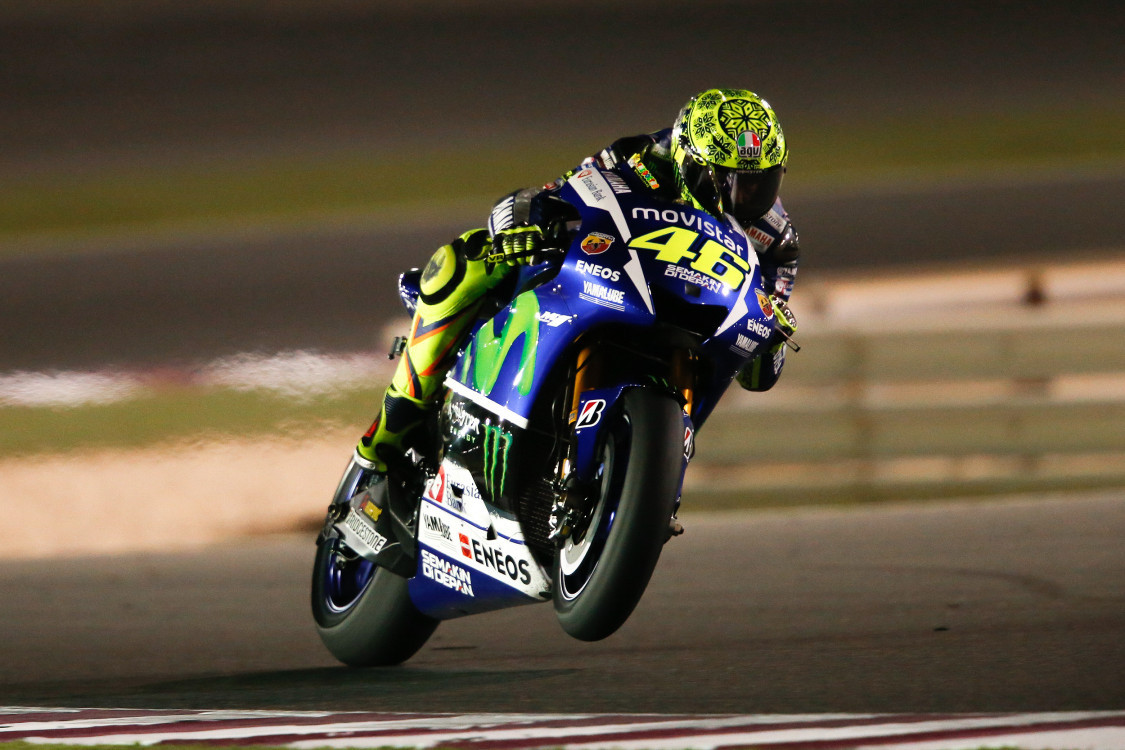
\includegraphics[width=0.45\textwidth]{wheelie1.jpg}
    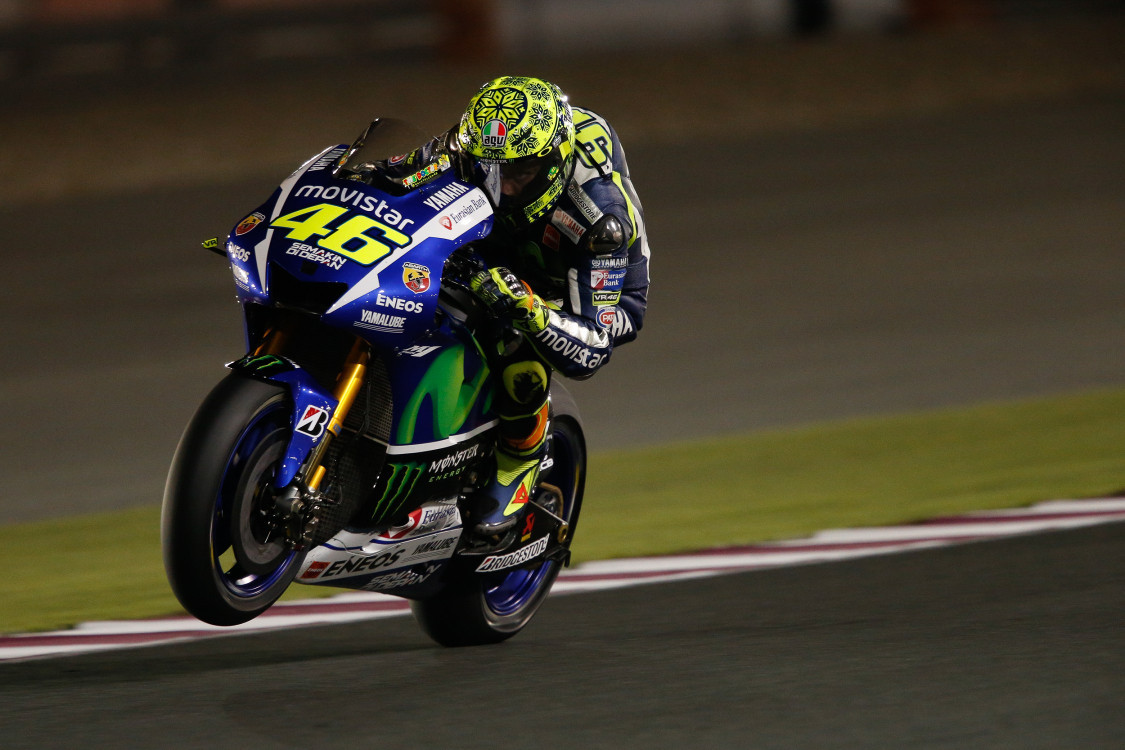
\includegraphics[width=0.45\textwidth]{wheelie2.jpg} \\
    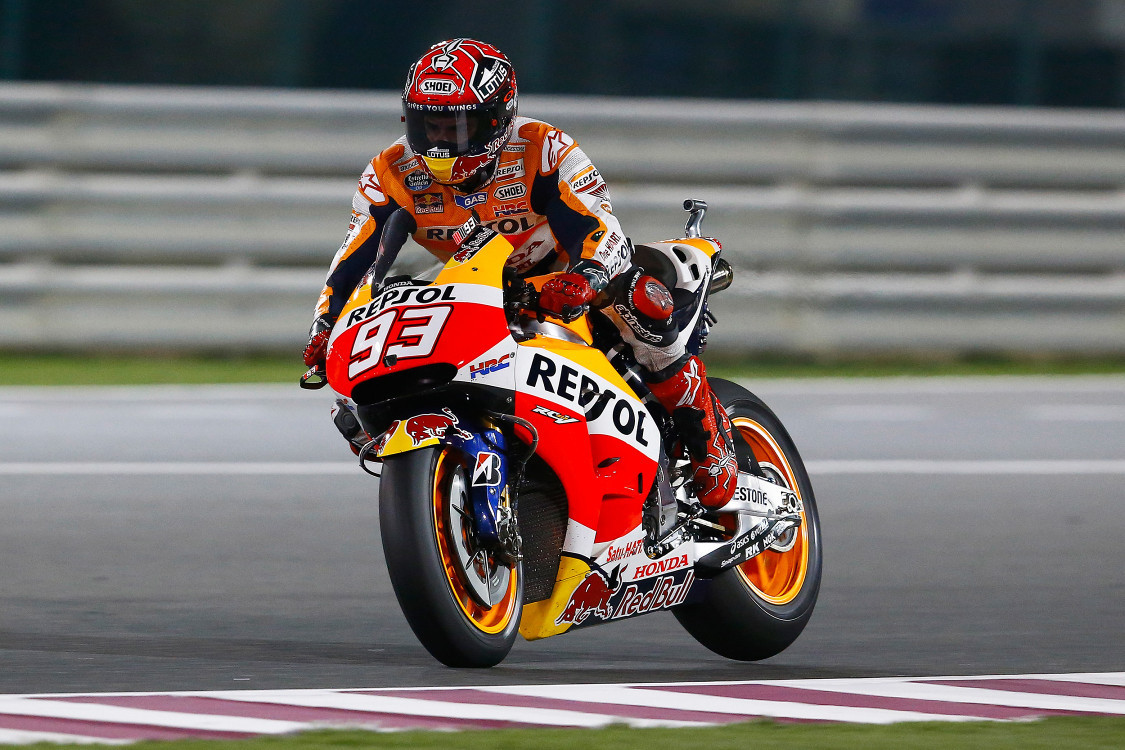
\includegraphics[width=0.45\textwidth]{stoppie.jpg}
    \caption[]{Top: two examples of a wheelie in a motorcycle race. When a wheelie happens, the rider generally does not decrease throttle, but rather uses the rear brake to control the pitch of the motorcycle. Bottom: a stoppie. In the bottom figure, notice that the motorcycle is trying to swivel around the steering axis: the rear is breaking out. If the rider reduces brake pressure too quickly, the rear will come down violently and cause a strong sideways vibration along the length axis of the motorcycle, which is very dangerous. These figures have a resolution of $1125 \times 750$ pixels. To maintain a resolution of at least 300 dpi, these figures should be printed no larger than $3.75 \times 2.5$ inches ($9.53 \times 6.35~\si{\centi\meter}$).}\label{fig::wheelie}
  \end{center}
\end{figure}

One of the weak points of \LaTeX\ is that it is not WYSIWYG (What You See Is What You Get), and it is, in general, not very easy to make schematics, diagrams, graphs, etc. In practice, one often uses a different software to make diagrams (perhaps even, oh horror!, PowerPoint), and then the diagram is included as a PDF file in the \LaTeX\ manuscript. This is not very satisfactory for two reasons: first, it's just not very practical from a management point of view, because if you want to change the diagram, you have to start the other software, remake the image, put in \LaTeX, judge if it's OK, and repeat, if needed. The other problem is that the fonts in the diagram will not be the same as in the text, and in many cases, once the image is properly scaled to fit into the manuscript, one finds out that the fonts have become either too small or too large.

\LaTeX\  offers a solution: PGF/TikZ. This package allows to make (2D) drawings in \LaTeX, and it is very flexible and very powerful. It can be used to make flow charts, mind-maps, but also graphs (similar to \texttt{GNUplot}). The advantage is that the scaling of the figure is automatically linked to the main \LaTeX\ file, the fonts are automatically taken care of, and you only have one input file to manage rather than using an external software tool. For example, in Figures~\ref{fig::ecco} and~\ref{fig::monju} are illustrated two examples of schematics created with PGF/TikZ. PGF/TikZ has a detailed manual (called \texttt{pgfmanual.pdf}), and this manual should be available on your computer if your \LaTeX-distribution contains the PGF/TikZ software.

\begin{figure}
  \begin{center}
    %\documentclass[a4paper,10pt]{revtex4-1}
%\usepackage{tikz}

%\begin{document}

%\thispagestyle{empty}

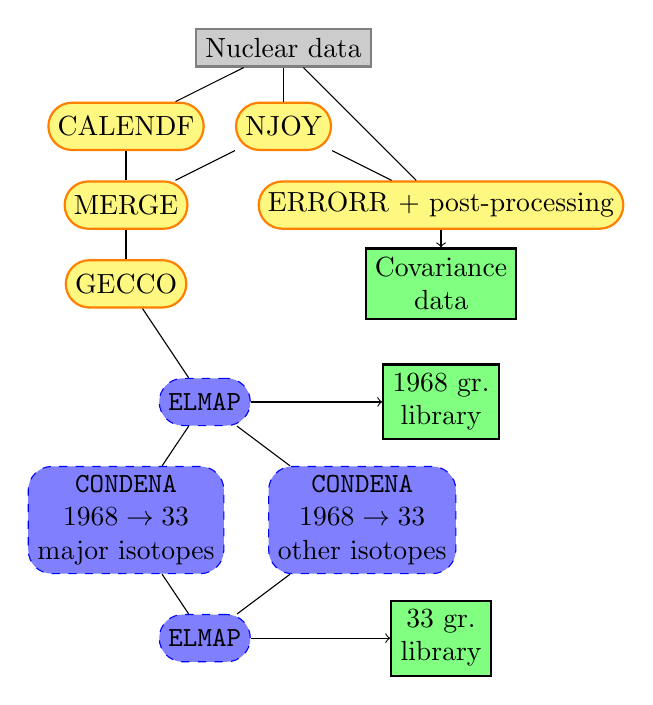
\begin{tikzpicture}[scale=1.0,
  data/.style={rectangle,draw=black!50,fill=black!20,thick},
  code/.style={rectangle,minimum size=6mm,rounded corners=3mm,fill=yellow!50,draw=orange,thick},
  lib/.style={rectangle,fill=green!50,draw=black,thick},
  emod/.style={rectangle,minimum size=6mm,rounded corners=3mm,fill=blue!50,draw=blue,dashed}]

  \pgfmathsetmacro{\ysep}{-1.0} ;
  
  \node[data] at ( 2, 0)       (nucdat)  {Nuclear data} ;
  \node[code] at ( 0, 1*\ysep) (calendf) {CALENDF} ;
  \node[code] at ( 2, 1*\ysep) (njoy1)   {NJOY}    ; 
  \node[code] at ( 0, 2*\ysep) (merge)   {MERGE}   ;
  \node[code] at ( 4, 2*\ysep) (errorr)  {ERRORR + post-processing}    ;
  \node[code] at ( 0, 3*\ysep) (gecco)   {GECCO}   ;
  \node[lib,align=center]  at ( 4, 3*\ysep) (cov)   {Covariance\\data} ;
  \node[emod] at ( 1, 4.5*\ysep) (elmap1)  {\texttt{ELMAP}}   ;
  \node[lib,align=center]  at ( 4, 4.5*\ysep) (lib1968)  {1968 gr.\\library}   ;
  \node[emod,align=center] at ( 0, 6*\ysep) (condena1)  {\texttt{CONDENA}\\$1968\rightarrow 33$\\major isotopes}   ;
  \node[emod,align=center] at ( 3, 6*\ysep) (condena2)  {\texttt{CONDENA}\\$1968\rightarrow 33$\\other isotopes}   ;
  \node[emod] at ( 1, 7.5*\ysep) (elmap2)  {\texttt{ELMAP}}   ;
  \node[lib,align=center]  at ( 4, 7.5*\ysep) (lib33)  {33 gr.\\library}   ;

  \draw[]   (nucdat)   -- (calendf) ;
  \draw[]   (nucdat)   -- (njoy1) ;
  \draw[]   (nucdat)   -- (errorr) ;
  \draw[]   (njoy1)    -- (errorr) ;
  \draw[]   (njoy1)    -- (merge) ;
  \draw[->] (errorr)   -- (cov) ;
  \draw[]   (calendf)  -- (merge) ;
  \draw[]   (merge)    -- (gecco) ;
  \draw[]   (gecco)    -- (elmap1) ;
  \draw[->] (elmap1)   -- (lib1968) ;
  \draw[]   (elmap1)   -- (condena1) ;
  \draw[]   (elmap1)   -- (condena2) ;
  \draw[]   (condena1) -- (elmap2) ;
  \draw[]   (condena2) -- (elmap2) ;
  \draw[->] (elmap2)   -- (lib33) ;

\end{tikzpicture}

%\end{document}


    \caption[]{Flow chart illustrating the steps required to make a cross section library for the ECCO code in ERANOS v2.0.}\label{fig::ecco}
  \end{center}
\end{figure}

\begin{figure}
  \begin{center}
    %------------------------------------------------------------------------------
% PGF/TikZ diagram of the Monju core. The basic approach is as follows:
% - the SAs are represented by nodes with a hexagonal shape
% - the pitch between SAs determines the size of the hexagons (using the inner
%   sep parameter)
% - for the major SA types there is a predefined color
% - the core has 60 degree symmetry, so use the rotation capability of PGF/TikZ
%   to determine the location of each SA
% - draw the diagram of the basic regions first
% - then overlay the "special cases"
% - LaTeX is not very good for calculations, and as a result, this kind of dia-
%   gram takes some time to compile (for example, each SA position must be
%   calculated, then a hexagon needs to be calculated around that position, etc)
%------------------------------------------------------------------------------

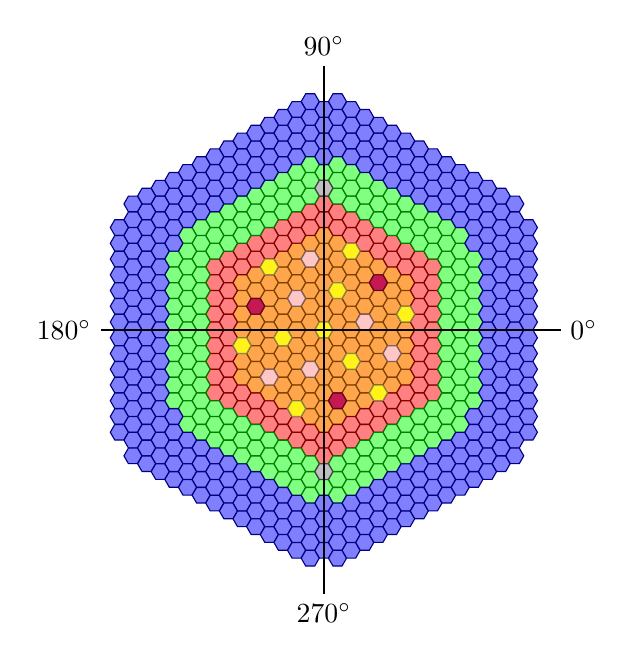
\begin{tikzpicture}[scale=1,
  default hexagon/.style={regular polygon, regular polygon sides=6, draw, 
  inner sep=0.07cm, fill=white, draw=white},
  reflector/.style={default hexagon, fill=blue!50!white, draw=blue!50!black},
  blanket/.style={default hexagon, fill=green!50!white, draw=green!50!black},
  outer fuel/.style={default hexagon, fill=red!50!white, draw=red!50!black},
  inner fuel/.style={default hexagon, fill=orange!70!white, draw=orange!50!black},
  ccr/.style={default hexagon, fill=yellow!90!white, draw=yellow!50!black},
  bcr/.style={default hexagon, fill=pink!90!white, draw=pink!50!black},
  fcr/.style={default hexagon, fill=purple!90!white, draw=purple!50!black},
  source/.style={default hexagon, fill=gray!50!white, draw=gray!50!black}
  ]

  \pgfmathsetmacro{\pitch}{0.2}

  %----------------------------------------------------------------------------
  % First ring
  %----------------------------------------------------------------------------
  \foreach \i in {0,...,5}{
    \node[inner fuel] at (\i * 60 + 30: \pitch) {} ;
  }
  
  %----------------------------------------------------------------------------
  % Remainder of inner fuel region
  %----------------------------------------------------------------------------
  \foreach \r in {2,...,6}{
    \foreach \i in {0,...,5}{
      \node[inner fuel] at (\i * 60 + 30: \r * \pitch) {} ;
      \pgfmathsetmacro{\rmo}{\r-1}
      \foreach \rr in {1,...,\rmo}{
        \draw ++(\i * 60 + 30: \r * \pitch)  +(\i * 60 + 150: \rr * \pitch) 
          node[inner fuel] {} ;      
      }
    }
  }

  %----------------------------------------------------------------------------
  % Outer fuel region
  %----------------------------------------------------------------------------
  \foreach \r in {7,8}{
    \foreach \i in {0,...,5}{
      \node[outer fuel] at (\i * 60 + 30: \r * \pitch) {} ;
      \pgfmathsetmacro{\rmo}{\r-1}
      \foreach \rr in {1,...,\rmo}{
        \draw ++(\i * 60 + 30: \r * \pitch)  +(\i * 60 + 150: \rr * \pitch) 
          node[outer fuel] {} ;      
      }
    }
  }

  %----------------------------------------------------------------------------
  % Blanket region
  %----------------------------------------------------------------------------
  \foreach \r in {9,...,11}{
    \foreach \i in {0,...,5}{
      \node[blanket] at (\i * 60 + 30: \r * \pitch) {} ;
      \pgfmathsetmacro{\rmo}{\r-1}
      \foreach \rr in {1,...,\rmo}{
        \draw ++(\i * 60 + 30: \r * \pitch)  +(\i * 60 + 150: \rr * \pitch) 
          node[blanket] {} ;      
      }
    }
  }

  %----------------------------------------------------------------------------
  % Reflector region
  %----------------------------------------------------------------------------
  \foreach \r in {12,...,14}{
    \foreach \i in {0,...,5}{
      \node[reflector] at (\i * 60 + 30: \r * \pitch) {} ;
      \pgfmathsetmacro{\rmo}{\r-1}
      \foreach \rr in {1,...,\rmo}{
        \draw ++(\i * 60 + 30: \r * \pitch)  +(\i * 60 + 150: \rr * \pitch) 
          node[reflector] {} ;      
      }
    }
  }

  %----------------------------------------------------------------------------
  % Reflector region last ring, missing 6 assemblies
  %----------------------------------------------------------------------------
  \foreach \r in {15,...,15}{
    \foreach \i in {0,...,5}{
      \pgfmathsetmacro{\rmo}{\r-1}
      \foreach \rr in {1,...,\rmo}{
        \draw ++(\i * 60 + 30: \r * \pitch)  +(\i * 60 + 150: \rr * \pitch) 
          node[reflector] {} ;      
      }
    }
  }

  %----------------------------------------------------------------------------
  % Neutron sources (2 SAs)
  %----------------------------------------------------------------------------
  \node[source] at (90:  9 *\pitch) {} ;
  \node[source] at (270:  9 *\pitch) {} ;

  %----------------------------------------------------------------------------
  % 6 reflectors in blanket region
  %----------------------------------------------------------------------------
  \foreach \i in {0,...,5}{
    \node[reflector] at (\i * 60 + 30: 11 * \pitch) {} ;
  }

  %----------------------------------------------------------------------------
  % 10 coarse control rods
  %----------------------------------------------------------------------------
  \node[ccr] at (0,0) {} ;
  \draw ++(90: 2 * \pitch)  +(30: \pitch) node[ccr] {} ; 
  \draw ++(90: 4 * \pitch)  +(30: 2 * \pitch) node[ccr] {} ; 
  \draw ++(90: -1 * \pitch)  +(-30: 2 * \pitch) node[ccr] {} ; 
  \draw ++(90: -2 * \pitch)  +(-30: 4 * \pitch) node[ccr] {} ; 
  \draw ++(90: -2 * \pitch)  +(150: 3 * \pitch) node[ccr] {} ; 
  \draw ++(90: -4 * \pitch)  +(150: 6 * \pitch) node[ccr] {} ; 
  \draw ++(90: 2 * \pitch)  +(150: 4 * \pitch) node[ccr] {} ; 
  \draw ++(90: -2 * \pitch)  +(30: 6 * \pitch) node[ccr] {} ; 
  \draw ++(90: -6 * \pitch)  +(150: 2 * \pitch) node[ccr] {} ; 

  %----------------------------------------------------------------------------
  % 6 backup rods
  %----------------------------------------------------------------------------
  \draw ++(90: 4 * \pitch)  +(150: \pitch) node[bcr] {} ; 
  \draw ++(90: \pitch)  +(150: 2 * \pitch) node[bcr] {} ; 
  \draw ++(90: -3 * \pitch)  +(150: \pitch) node[bcr] {} ; 
  \draw ++(90: -5 * \pitch)  +(150: 4 * \pitch) node[bcr] {} ; 
  \draw ++(90: -1 * \pitch)  +(30: 3 * \pitch) node[bcr] {} ; 
  \draw ++(90: -4 * \pitch)  +(30: 5 * \pitch) node[bcr] {} ; 

  %----------------------------------------------------------------------------
  % 3 fine control rods
  %----------------------------------------------------------------------------
  \draw ++(90: 1 * \pitch)  +(30: 4 * \pitch) node[fcr] {} ; 
  \draw ++(90: -1 * \pitch)  +(150: 5 * \pitch) node[fcr] {} ; 
  \draw ++(90: -5 * \pitch)  +(30: \pitch) node[fcr] {} ; 

  \node[](AA) at ( -3.3,  0 ) {\SI{180}{\degree}};
  \node[](BB) at (  3.3,  0 ) {\SI{0}{\degree}} ;
  \node[](CC) at (   0, 3.6 ) {\SI{90}{\degree}}  ;
  \node[](DD) at (   0,-3.6 ) {\SI{270}{\degree}} ;
  \draw[thick] (AA) -- (BB) ;
  \draw[thick] (CC) -- (DD) ;
\end{tikzpicture}


    \caption[]{Layout of the MONJU core. PGF/TikZ allows the use of loops and color-codings to make it somewhat easier to automatically generate such diagrams. All distances are calculated, so that the grid of hexagons looks good under any magnification.}\label{fig::monju}
  \end{center}
\end{figure}

%------------------------------------------------------------------------------
%
%------------------------------------------------------------------------------
\section{CONCLUSION} 
\label{sect::conclusion}

Concluding: good luck with the preparation of your manuscript.

%------------------------------------------------------------------------------
%
%------------------------------------------------------------------------------
\section*{ACKNOWLEDGMENTS}

If you want to thank somebody or something (maybe a funding organisation), do it here.

%------------------------------------------------------------------------------
% Bibliography. There are two ways to include the bibliography in your manu-
% script: 
% 1. use BibTeX: put physor2014.bst in your working directory  -or-
% 2. Manual list of references
% BibTeX is the preferred method, as it will take care of sorting etc automa-
% tically. To use BibTeX you need to make a database (.bib file), see the 
% example in the template. Many programs are available to make a BibTeX data-
% base for you, for example:
% - PyBliographer (http://www.pybliographer.org/)
% - Jabref        (http://jabref.sourceforge.net/)
%
% For BibTeX users: include as many bibliographic details as possible. The 
% physor2014.bst style file will select the relevant fields from your .bib file.
% Most bibliographic data are optional; if a required entry is missing BibTeX
% will complain about it.
% The physor2014.bst file allows the following non-standard options
% - a "doi" field, which will show as http://dx.doi.org/doi_number
% - a "url" field, which will set URLs in the proper way
% - the doi and url fields are processed by hyperref and result in clickable 
%   links
%
% In all cases (both for manual entry and for bibtex): 
% - The authors full name is preferred over initials (i.e. "Mercedes Benz" is 
%   preferred over "M. Benz")
% - List a maximum of three authors, separated by commas. If there are more than
%   threee authors, use "First Author \emph{et al},"
% - List as much bibliographic details as possible but if data are missing then
%   just leave the entries blank
%
% If you use BibTeX: 
%
\bibliographystyle{physor2016}
\bibliography{physor2016}
%
% If you use manual input, use the following format.
%------------------------------------------------------------------------------
% \begin{thebibliography}{300}
% \bibitem{journal} Some Author(s), ``Article Title,'' \emph{Journal Name}, \textbf{Volume(number)}: pp. 34-89 URL \url{http://dx.doi.org/doi_number} (19xx).
%
% \bibitem{proc_paper} C. D. Author(s), ``Article Title,'' In: \emph{Proceedings of Meeting} (Editor Name, editor), Organisation, Location, Dates of Meeting, Vol. n: pp. 134-156 (19xx).
%
% \bibitem{book} Epsilon F. Author, \emph{Book Title in Italic}, Publisher, City \& Country (19xx). 
%
% \bibitem{website} ``Research Institute of Nuclear Engineering, University of Fukui'', \url{http://www.rine.u-fukui.ac.jp/english/index.html} (2013).
% \end{thebibliography}
%
%------------------------------------------------------------------------------
% Set up for appendices
%------------------------------------------------------------------------------
\appendix

\makeatletter
\def\@seccntformat#1{APPENDIX \csname the#1\endcsname.~}
\makeatother

%------------------------------------------------------------------------------
% If you need to make one (or more) appendix (appendices), place them here as
% sections
%------------------------------------------------------------------------------
\section{HOW TO MAKE APPENDICES}
\label{app::a}

An appendix is a section with extra material which is relevant to the manuscript, but is too bulky, too detailed, or simply too long to include in the main text. Feel free to make one (or more) appendix (appendices), but remember: if you make an appendix, then you must include a reference from the main text to the appendix. An unreferenced (``dangling") appendix is not allowed.

\section{ISSUES RELATED TO FISSION PRODUCT DECOUPLING IN ADJOINT TRANSMUTATION CALCULATIONS}
\label{app::b}

An appendix is a section with extra material which is relevant to the manuscript, but is too bulky, too detailed, or simply too long to include in the main text. Feel free to make one (or more) appendix (appendices), but remember: if you make an appendix, then you must include a reference from the main text to the appendix. An unreferenced (``dangling") appendix is not allowed.

\end{document}

%------------------------------------------------------------------------------
% pdflatex allows figures in PDF, JPG and PNG. For users who have prepared their
% figures in (e)ps, please find here some tips and tricks:
% - Nearly all latex distributions have the tool "ps2pdf". This tool translates 
%   (e)ps files into pdf files, which can be included in pdflatex
%
%   Usage:
%
%   rooijen@vogsphere ~> ps2pdf file.eps
%
% - In some cases, ps2pdf produces a pdf file on a4 size (or US letter size, de-
%   pending on your computer's settings) with a lot of white space around the
%   figure. In such a case, use "pdfcrop" to cut  off the excess white space.
%
%   Usage:
%
%   rooijen@vogsphere ~> pdfcrop file.pdf
%
%   The new file will be called file-crop.pdf
%
% - If you have very many (e)ps files that need conversion, consider making a 
%   BASH script or something similar and use ps2pdf and pdfcrop on each (e)ps
%   file
%------------------------------------------------------------------------------

